\chapter{Array dan ArrayList}

\section{Array dan ArrayList di Java}

\subsection{Array}

Array adalah struktur data yang menyimpan sekumpulan elemen dengan tipe yang sama dalam urutan tertentu. Array memiliki ukuran tetap yang ditentukan saat deklarasi. Beberapa karakteristik array di Java adalah:

\begin{itemize}
	\item \textbf{Deklarasi dan Inisialisasi:} Array dapat dideklarasikan dengan menyebutkan tipe data diikuti oleh nama array dan ukuran array. Contoh:
	\begin{lstlisting}[style=JavaStyle]
		int[] numbers = new int[5];
	\end{lstlisting}
	Array dapat diinisialisasi dengan nilai-nilai pada saat deklarasi:
	\begin{lstlisting}[style=JavaStyle]
		int[] numbers = {1, 2, 3, 4, 5};
	\end{lstlisting}
	\item \textbf{Akses Elemen:} Elemen array diakses menggunakan indeks, yang dimulai dari 0:
	\begin{lstlisting}[style=JavaStyle]
		int firstNumber = numbers[0]; // Mengakses elemen pertama
	\end{lstlisting}
	\item \textbf{Ukuran Array:} Ukuran array tetap dan dapat diakses dengan menggunakan \texttt{length}:
	\begin{lstlisting}[style=JavaStyle]
		int size = numbers.length;
	\end{lstlisting}
\end{itemize}

\subsection{ArrayList}

`ArrayList` adalah implementasi dari interface `List` yang menggunakan array dinamis untuk menyimpan elemen. Beberapa karakteristik `ArrayList` di Java adalah:

\begin{itemize}
	\item \textbf{Deklarasi dan Inisialisasi:} `ArrayList` dapat dideklarasikan dan diinisialisasi dengan tipe data generik. Contoh:
	\begin{lstlisting}[style=JavaStyle]
		ArrayList<Integer> list = new ArrayList<>();
	\end{lstlisting}
	\item \textbf{Menambahkan dan Mengakses Elemen:} Elemen dapat ditambahkan dengan metode \texttt{add} dan diakses dengan metode \texttt{get}:
	\begin{lstlisting}[style=JavaStyle]
		list.add(10);
		int element = list.get(0);
	\end{lstlisting}
	\item \textbf{Menghapus Elemen:} Elemen dapat dihapus dengan metode \texttt{remove}:
	\begin{lstlisting}[style=JavaStyle]
		list.remove(0); // Menghapus elemen pada indeks 0
	\end{lstlisting}
	\item \textbf{Ukuran ArrayList:} Ukuran `ArrayList` dapat diakses dengan menggunakan metode \texttt{size}:
	\begin{lstlisting}[style=JavaStyle]
		int size = list.size();
	\end{lstlisting}
\end{itemize}

\subsection{Konversi Antara Array dan ArrayList}

Mengonversi antara `Array` dan `ArrayList` memungkinkan fleksibilitas dalam manipulasi data. Berikut adalah metode umum untuk konversi:

\begin{itemize}
	\item \textbf{ArrayList ke Array:} Gunakan metode \texttt{toArray(T[] a)} atau stream untuk mengonversi `ArrayList` menjadi array:
	\begin{lstlisting}[style=JavaStyle]
		Integer[] array = list.toArray(new Integer[0]);
		Integer[] array2 = list.stream().toArray(Integer[]::new);
	\end{lstlisting}
	\item \textbf{Array ke ArrayList:} Gunakan metode \texttt{Arrays.asList(T... a)} untuk mengonversi array menjadi `ArrayList`:
	\begin{lstlisting}[style=JavaStyle]
		ArrayList<Integer> newList = new ArrayList<>(Arrays.asList(array));
	\end{lstlisting}
\end{itemize}

\section{Penggunaan Array di Java}

\begin{lstlisting}[style=JavaStyle]
	package org.alfa.pertemuan06.arrayandlist;
	
	import java.util.Arrays;
	
	public class ArrayDemo {
		public static void main(String[] args) {
			int[] a = null;
			int[] b = new int[] {};
			int[] c = { 1, 2, 3 };
			double[] d = new double[] { 1, 2, 3, 4 };
			double[] e = Arrays.copyOfRange(d, 1, 4);
			
			System.out.println(Arrays.toString(a));
			System.out.println(Arrays.toString(b));
			System.out.println(Arrays.toString(c));
			System.out.println(Arrays.toString(d));
			System.out.println(Arrays.toString(e));
			
			System.out.print(d[0]);
			System.out.print(", " + d[1]);
			System.out.print(", " + d[3]);
			
			int[] f = new int[3];
			f[2] = 99;
			f[1] = 100;
			f[0] = 31;
			
			System.out.print(f[0]);
			System.out.print(", " + f[1]);
			System.out.print(", " + f[2]);
		}
	}
\end{lstlisting}

\subsection{Pembahasan}

\subsubsection{Deklarasi dan Inisialisasi Array}

Dalam kode di atas, beberapa array dideklarasikan dan diinisialisasi dengan cara yang berbeda:

\begin{itemize}
	\item \textbf{Array \texttt{a}:} Dideklarasikan tetapi tidak diinisialisasi, sehingga nilainya \texttt{null}.
	\item \textbf{Array \texttt{b}:} Dideklarasikan dan diinisialisasi sebagai array kosong. \texttt{b.length} akan mengembalikan \texttt{0}.
	\item \textbf{Array \texttt{c}:} Dideklarasikan dan diinisialisasi dengan tiga elemen \{1, 2, 3\}.
	\item \textbf{Array \texttt{d}:} Dideklarasikan dan diinisialisasi dengan empat elemen \{1, 2, 3, 4\}.
	\item \textbf{Array \texttt{e}:} Dibuat dengan menggunakan metode \texttt{Arrays.copyOfRange()} untuk menyalin elemen dari indeks 1 hingga 3 dari array \texttt{d}. Ini akan menghasilkan array \{2, 3, 4\}.
\end{itemize}

\subsubsection{Pencetakan Array}

Kode diatas menunjukkan beberapa cara untuk mencetak elemen array:
\begin{itemize}
	\item \texttt{System.out.println(Arrays.toString(array))}: Digunakan untuk mencetak elemen array dalam format string yang terpisah oleh koma.
	\item \texttt{System.out.print()}: Digunakan untuk mencetak elemen array satu per satu dengan pemisah yang ditentukan.
\end{itemize}

\subsubsection{Inisialisasi dan Pencetakan Array Baru}

\begin{itemize}
	\item \textbf{Array \texttt{f}:} Dideklarasikan dengan ukuran 3 dan diinisialisasi dengan nilai \{31, 100, 99\}.
	\item \texttt{System.out.print(f[0]); System.out.print(", " + f[1]); System.out.print(", " + f[2]);}: Digunakan untuk mencetak elemen-elemen array \texttt{f} dengan pemisah koma.
\end{itemize}

\section{Penggunaan ArrayList di Java}

\begin{lstlisting}[style=JavaStyle]
	package org.alfa.pertemuan06.arrayandlist;
	
	import java.util.ArrayList;
	import java.util.Arrays;
	
	public class ArrayListDemo {
		public static void main(String[] args) {
			ArrayList<Integer> a = null;
			ArrayList<Integer> b = new ArrayList<Integer>();
			ArrayList<Integer> c = 
			new ArrayList<>(Arrays.asList(73, 101, 6));
			
			b.add(99);
			System.out.println(b);
			b.add(97);
			b.add(0, 98);
			System.out.println(b);
			b.add(97);
			System.out.println(b);
			
			System.out.println("b's Size = " + b.size());
			
			b.remove(0);
			System.out.println(b);
			
			b.remove(97);
			Integer z = 97;
			b.remove(z);
			System.out.println(b);
			
			System.out.println("c(0) = " + c.get(0));
			System.out.println("c(2) = " + c.get(c.size() - 1));
			
			System.out.println(c);
			c.add(1, 999);
			System.out.println("c(0) = " + c.get(0));
			System.out.println("c(1) = " + c.get(1));
			System.out.println(c);
		}
	}
\end{lstlisting}

\subsection{Pembahasan}

\subsubsection{Deklarasi dan Inisialisasi ArrayList}

Dalam kode di atas, beberapa `ArrayList` dideklarasikan dan diinisialisasi dengan cara yang berbeda:

\begin{itemize}
	\item \textbf{ArrayList \texttt{a}:} Dideklarasikan tetapi tidak diinisialisasi, sehingga nilainya \texttt{null}.
	\item \textbf{ArrayList \texttt{b}:} Dideklarasikan dan diinisialisasi sebagai `ArrayList` kosong.
	\item \textbf{ArrayList \texttt{c}:} Dideklarasikan dan diinisialisasi dengan tiga elemen \{73, 101, 6\} menggunakan metode \texttt{Arrays.asList()}.
\end{itemize}

\subsubsection{Operasi pada ArrayList}

Kode diatas menunjukkan beberapa operasi dasar dengan `ArrayList`:

\begin{itemize}
	\item \texttt{add(element)}: Menambahkan elemen ke dalam `ArrayList`. Misalnya, \texttt{b.add(99)} menambahkan nilai 99 ke dalam `b`.
	\item \texttt{add(index, element)}: Menambahkan elemen pada posisi tertentu. Misalnya, \texttt{b.add(0, 98)} menambahkan nilai 98 di posisi indeks 0.
	\item \texttt{remove(index)}: Menghapus elemen pada posisi tertentu. Misalnya, \texttt{b.remove(0)} menghapus elemen pada indeks 0.
	\item \texttt{remove(element)}: Menghapus elemen yang spesifik. Misalnya, \texttt{b.remove(z)} menghapus nilai yang sama dengan nilai variabel \texttt{z}.
	\item \texttt{size()}: Mengembalikan jumlah elemen dalam `ArrayList`. Misalnya, \texttt{b.size()} mengembalikan ukuran dari `b`.
\end{itemize}

\subsubsection{Mengakses dan Memodifikasi Elemen}

\begin{itemize}
	\item \textbf{Mengakses Elemen:} Elemen `ArrayList` dapat diakses menggunakan metode \texttt{get(index)}. Misalnya, \texttt{c.get(0)} mengakses elemen pertama dari `c`.
	\item \textbf{Modifikasi Elemen:} Elemen `ArrayList` dapat dimodifikasi menggunakan metode \texttt{add(index, element)}. Misalnya, \texttt{c.add(1, 999)} menambahkan nilai 999 di posisi indeks 1.
\end{itemize}

\subsubsection{Array of Objects}

Bagian kode yang dikomentari juga menunjukkan penggunaan array objek. `Object[]` dapat digunakan untuk menyimpan berbagai tipe objek:

\begin{itemize}
	\item \textbf{Array \texttt{person}:} Dideklarasikan dengan ukuran 10 dan diisi dengan nilai yang berbeda, termasuk `String` dan `Double`.
	\item \textbf{Array \texttt{people}:} Dideklarasikan dengan ukuran 100 dan diisi dengan array \texttt{person}.
\end{itemize}

\section{Konversi Antara Array dan ArrayList di Java}

\begin{lstlisting}[style=JavaStyle]
	package org.alfa.pertemuan06.arrayandlist;
	
	import java.util.ArrayList;
	import java.util.Arrays;
	
	public class Coversion {
		public static void main(String[] args) {
			ArrayList<Integer> list = new ArrayList<>();
			list.add(3);
			list.add(2);
			list.add(1);
			System.out.println("List: " + list);
			
			Integer[] array = list.toArray(new Integer[0]);
			System.out.println("Array 1: " + Arrays.toString(array));
			
			Integer[] array2 = list.stream().toArray(Integer[]::new);
			System.out.println("Array 2: " + Arrays.toString(array2));
			
			ArrayList<Integer> newList = new ArrayList<>(Arrays.asList(array));
			System.out.println("New List: " + newList);
			
			int[] a = new int[list.size()];
			a[2] = list.get(0); 
			a[1] = list.get(1); 
			a[0] = list.get(2);
			System.out.println("Array a: " + Arrays.toString(a));
			
			ArrayList<Integer> l = new ArrayList<>();
			l.add(a[2]);
			l.add(a[1]);
			l.add(a[0]);
			System.out.println("List l: " + l.toString());
		}
	}
\end{lstlisting}

\subsection{Pembahasan}

\subsubsection{Konversi dari ArrayList ke Array}

Beberapa metode untuk mengonversi `ArrayList` ke array ditunjukkan dalam kode:

\begin{itemize}
	\item \textbf{Metode \texttt{toArray(T[] a)}:} Mengonversi `ArrayList` menjadi array dengan jenis yang sama. Misalnya, \texttt{list.toArray(new Integer[0])} mengonversi `list` menjadi array \texttt{Integer}.
	\item \textbf{Metode Stream \texttt{toArray()} :} Menggunakan stream untuk mengonversi `ArrayList` menjadi array. Misalnya, \texttt{list.stream().toArray(Integer[]::new)} mengonversi `list` menjadi array \texttt{Integer[]}.
\end{itemize}

\subsubsection{Konversi dari Array ke ArrayList}

\begin{itemize}
	\item \textbf{Metode \texttt{Arrays.asList(T... a)}:} Mengonversi array menjadi `ArrayList`. Misalnya, \texttt{new ArrayList<>(Arrays.asList(array))} mengonversi array \texttt{array} menjadi `ArrayList`.
\end{itemize}

\subsubsection{Manipulasi Array dan ArrayList}

\begin{itemize}
	\item \textbf{Array dari List:} Membuat array \texttt{int} dan menyalin elemen dari `ArrayList` ke array tersebut. Misalnya, \texttt{a[2] = list.get(0)} menyalin elemen pertama dari `list` ke posisi ketiga dari array \texttt{a}.
	\item \textbf{List dari Array:} Membuat `ArrayList` baru dari array \texttt{int}. Misalnya, \texttt{l.add(a[2])} menambahkan elemen array ke dalam `ArrayList`.
\end{itemize}

\section{Latihan dan Contoh Kode}

Berikut adalah beberapa latihan untuk membantu Anda memahami penggunaan Array, ArrayList, dan konversi di Java.

\begin{enumerate}
	
	\item \textbf{Latihan 1: Mengelola Data Mahasiswa}
	
	Tugas: Buatlah sebuah program yang mengelola data mahasiswa dengan menggunakan \texttt{ArrayList}. Tambahkan nama mahasiswa ke dalam list, cetak semua nama, hapus nama tertentu, dan cetak ukuran list setelah penghapusan.
	
	\begin{lstlisting}[style=JavaStyle]
		package org.alfa.pertemuan06.arrayandlist;
		
		import java.util.ArrayList;
		
		public class StudentListDemo {
			
			public static void main(String[] args) {
				ArrayList<String> students = new ArrayList<>();
				students.add("Alice");
				students.add("Bob");
				students.add("Charlie");
				
				System.out.println("Students: " + students);
				
				students.remove("Bob");
				System.out.println("Students after removal: " + students);
				System.out.println("Number of students: " + students.size());
			}
		}
	\end{lstlisting}
	
	\item \textbf{Latihan 2: Konversi Array ke ArrayList dan Sebaliknya}
	
	Tugas: Buatlah program yang mengonversi array string menjadi \texttt{ArrayList}, tambahkan beberapa elemen ke \texttt{ArrayList}, konversi kembali ke array, dan cetak hasilnya.
	
	\begin{lstlisting}[style=JavaStyle]
		package org.alfa.pertemuan06.arrayandlist;
		
		import java.util.ArrayList;
		import java.util.Arrays;
		
		public class ConversionDemo {
			
			public static void main(String[] args) {
				String[] array = {"Red", "Green", "Blue"};
				ArrayList<String> list = new ArrayList<>(Arrays.asList(array));
				
				list.add("Yellow");
				list.add("Purple");
				
				String[] newArray = list.toArray(new String[0]);
				System.out.println("New Array: " + Arrays.toString(newArray));
			}
		}
	\end{lstlisting}
	
	\item \textbf{Latihan 3: Array Multi-Dimensi dan ArrayList}
	
	Tugas: Buatlah program yang menggunakan array dua dimensi untuk menyimpan nilai integer. Konversikan baris pertama dari array dua dimensi ke dalam \texttt{ArrayList}, kemudian cetak hasilnya.
	
	\begin{lstlisting}[style=JavaStyle]
		package org.alfa.pertemuan06.arrayandlist;
		
		import java.util.ArrayList;
		import java.util.Arrays;
		
		public class MultiDimArrayDemo {
			
			public static void main(String[] args) {
				int[][] matrix = {
					{1, 2, 3},
					{4, 5, 6},
					{7, 8, 9}
				};
				
				ArrayList<Integer> firstRow = new ArrayList<>();
				for (int num : matrix[0]) {
					firstRow.add(num);
				}
				
				System.out.println("First Row as ArrayList: " + firstRow); // First Row as ArrayList: [1, 2, 3]
			}
		}
	\end{lstlisting}
\end{enumerate}

\section{Soal}

Berikut adalah beberapa latihan yang berkaitan dengan penggunaan Array dan ArrayList di Java:

\begin{enumerate}
	
	\item \textbf{Soal 1:} Tulis program yang mengelola daftar tugas menggunakan \texttt{ArrayList}. Tambahkan beberapa tugas ke dalam daftar, tandai tugas sebagai selesai dengan menghapusnya dari daftar, dan cetak daftar tugas yang tersisa setelah beberapa tugas dihapus.
	
	\item \textbf{Soal 2:} Tulis program yang menginisialisasi array dua dimensi dengan nilai acak antara 1 hingga 100. Konversikan setiap baris dari array dua dimensi ke dalam \texttt{ArrayList}, lalu cetak \texttt{ArrayList} dari setiap baris.
	
	\item \textbf{Soal 3:} Tulis program yang mengelola daftar nilai siswa menggunakan \texttt{ArrayList} dengan tipe data \texttt{Double}. Tambahkan beberapa nilai ke dalam daftar, hitung rata-rata nilai, dan cetak daftar nilai yang lebih besar dari rata-rata tersebut.
	
\end{enumerate}

\section{Soal List}
Diberikan data mahasiswa berupa NIM, Nama, Umur, Mata Kuliah, dan Nilai. Gunakan bahasa pemrograman Java untuk menyelesaikan masalah berikut:

\begin{enumerate}
	\item \textbf{Buatlah Kelas untuk Merepresentasikan Data Mahasiswa di Memori} \\
	Buatlah dua kelas:
	\begin{itemize}
		\item Kelas \texttt{Mahasiswa} untuk merepresentasikan data mahasiswa yang mencakup NIM, Nama, dan Umur.
		\item Kelas \texttt{HasilUjian} untuk merepresentasikan hasil ujian mahasiswa yang mencakup NIM, Mata Kuliah, dan Nilai.
	\end{itemize}
	
	\item \textbf{Buatlah Fungsi untuk Mencari Umur Mahasiswa} \\
	Buat fungsi yang menerima NIM sebagai parameter dan mengembalikan umur mahasiswa.
	
	\item \textbf{Buat Fungsi untuk Mencari Mahasiswa Berdasarkan Jangkauan Umur} \\
	Buat fungsi yang menerima dua parameter (umur minimum dan maksimum) dan mengembalikan daftar mahasiswa yang berusia di antara dua nilai tersebut.
	
	\item \textbf{Buatlah Fungsi untuk Mencari Mata Kuliah dan Nilai Berdasarkan Nama Mahasiswa} \\
	Buat fungsi yang menerima nama mahasiswa sebagai parameter dan mengembalikan daftar mata kuliah beserta nilai ujian yang diambil oleh mahasiswa tersebut.
	
	\item \textbf{Buatlah Fungsi untuk Mencari Nilai Rata-Rata Ujian untuk Setiap Mahasiswa} \\
	Buat fungsi yang menerima NIM sebagai parameter dan mengembalikan nilai rata-rata ujian dari mahasiswa tersebut.
	
	\item \textbf{Cari Mahasiswa dengan Nilai Rata-Rata Paling Tinggi dan Paling Rendah} \\
	Buat fungsi yang mencari dan mengembalikan mahasiswa dengan nilai rata-rata ujian paling tinggi dan paling rendah.
	
	\item \textbf{Buatlah Normalisasi Data Nilai untuk Setiap Mata Kuliah} \\
	Buat fungsi untuk menormalisasi nilai setiap mata kuliah berdasarkan nilai tertinggi dan terendah pada mata kuliah tersebut. Cari di internet cara menormalisasikan data numerik.
	
	
\end{enumerate}

\subsection{Contoh Data (Sebagai Acuan untuk Implementasi)}

\textbf{Tabel 1: Data Mahasiswa}
\begin{verbatim}
	NIM       | Nama       | Umur
	-------------------------------
	123456789 | Alice      | 20   
	987654321 | Bob        | 22   
	192837465 | Charlie    | 21   
\end{verbatim}

\textbf{Tabel 2: Hasil Ujian}
\begin{verbatim}
	NIM       | Mata Kuliah         | Nilai
	----------------------------------------
	123456789 | Dasar Pemrograman   | 85   
	123456789 | Algoritma           | 78   
	987654321 | Dasar Pemrograman   | 90   
	987654321 | Algoritma           | 65   
	192837465 | Dasar Pemrograman   | 88   
	192837465 | Algoritma           | 73   
\end{verbatim}

\section{Soal \textit{Searching}}

Diberikan sebuah array yang berisi sejumlah angka acak. Tugas Anda adalah mengimplementasikan beberapa fungsi pencarian untuk melakukan operasi berikut:

\begin{enumerate}
	\item \textbf{Pencarian Nilai Tertentu} \\
	Buatlah fungsi yang menerima sebuah array integer dan sebuah nilai integer sebagai parameter, kemudian kembalikan \texttt{true} jika nilai tersebut ada dalam array, dan \texttt{false} jika tidak ada.
	
	\item \textbf{Pencarian Nilai Minimum} \\
	Buatlah fungsi yang menerima sebuah array integer sebagai parameter dan mengembalikan nilai minimum dari array tersebut. 
	
	\item \textbf{Pencarian Nilai Maksimum} \\
	Buatlah fungsi yang menerima sebuah array integer sebagai parameter dan mengembalikan nilai maksimum dari array tersebut.
	
	\item \textbf{Binary Search} \\
	Buatlah fungsi yang menerima sebuah array integer yang sudah diurutkan dan sebuah nilai integer sebagai parameter. Fungsi ini harus mengembalikan indeks dari nilai tersebut dalam array. Jika nilai tidak ditemukan, kembalikan -1.
\end{enumerate}

\subsection{Contoh Input}

Berikut adalah contoh array yang dapat Anda gunakan untuk pengujian:

\[
array = [64, 34, 25, 12, 22, 11, 90]
\]

Setelah mengurutkan array, hasilnya menjadi:

\[
array_{sorted} = [11, 12, 22, 25, 34, 64, 90]
\]

\subsection{Contoh Output}

Setelah menjalankan masing-masing fungsi, output yang diharapkan adalah:

\begin{itemize}
	\item \textbf{Output Pencarian Nilai Tertentu (22):} \texttt{true}
	\item \textbf{Output Pencarian Nilai Minimum:} 11
	\item \textbf{Output Pencarian Nilai Maksimum:} 90
	\item \textbf{Output Binary Search (nilai 34):} 4
	\item \textbf{Output Binary Search (nilai 100):} -1
\end{itemize}

\subsection{Petunjuk:}

\begin{itemize}
	\item Pastikan setiap fungsi menerima parameter array dan mengembalikan hasil yang sesuai dengan operasi pencarian yang diminta.
	\item Gunakan algoritma pencarian yang efisien untuk fungsi pencarian biner.
	\item Uji setiap fungsi dengan beberapa array dan nilai berbeda untuk memastikan bahwa algoritma berfungsi dengan baik.
\end{itemize}

Tugas Anda adalah mengimplementasikan fungsi-fungsi tersebut dalam bahasa pemrograman Java.


\section{Soal Sorting}

Diberikan sebuah array yang berisi sejumlah angka acak. Tugas Anda adalah mengimplementasikan tiga algoritma pengurutan, yaitu \textit{Insertion Sort}, \textit{Selection Sort}, dan \textit{Bubble Sort}, untuk mengurutkan array tersebut. Buatlah fungsi yang menerima sebuah array integer sebagai parameter dan mengurutkan array tersebut menggunakan algoritma Insertion Sort. Setelah array diurutkan, tampilkan array yang telah diurutkan.
Untuk pembelajaran lebih lanjut, coba lakukan hal yang sama untuk \textit{Quick Sort}.

\subsection{Contoh Input}

Berikut adalah contoh array yang dapat Anda gunakan untuk pengujian:

\[
array = [64, 34, 25, 12, 22, 11, 90]
\]

\subsection{Contoh Output}

Setelah menjalankan masing-masing algoritma pengurutan, output yang diharapkan adalah:

\begin{itemize}
	\item \textbf{Output Insertion Sort:} [11, 12, 22, 25, 34, 64, 90]
	\item \textbf{Output Selection Sort:} [11, 12, 22, 25, 34, 64, 90]
	\item \textbf{Output Bubble Sort:} [11, 12, 22, 25, 34, 64, 90]
\end{itemize}

\subsection{Petunjuk:}

\begin{itemize}
	\item Pastikan setiap fungsi pengurutan menerima parameter array dan mengubah array tersebut secara in-place (tanpa menggunakan array tambahan).
	\item Uji setiap fungsi dengan beberapa array berbeda untuk memastikan bahwa algoritma berfungsi dengan baik.
\end{itemize}

Tugas Anda adalah mengimplementasikan fungsi-fungsi tersebut dalam bahasa pemrograman Java.

\section{Soal \textit{Tree}}

Diberikan sebuah struktur organisasi perusahaan yang direpresentasikan menggunakan struktur data pohon (tree). Setiap node dalam pohon mewakili seorang karyawan, dan setiap karyawan memiliki bawahan langsung (child nodes) atau atasan (parent node). Anda diminta untuk mengimplementasikan beberapa fungsi untuk menavigasi dan mencari dalam struktur ini.


\begin{enumerate}
	\item \textbf{Mencari Atasan dari Karyawan Tertentu} \\
	Buatlah fungsi yang menerima nama seorang karyawan dan mengembalikan nama atasannya langsung (parent node) jika ada, atau null jika karyawan tersebut adalah atasan tertinggi (root node).
	
	\item \textbf{Mencari Atasan Hingga Atasan Paling Atas (CEO)} \\
	Buatlah fungsi yang menerima nama seorang karyawan dan mengembalikan daftar nama-nama atasannya mulai dari atasan langsung hingga ke atasan paling atas (root node/CEO). Jika karyawan tersebut adalah CEO, kembalikan daftar kosong.
	
	\item \textbf{Mencari Bawahan Langsung dari Karyawan Tertentu} \\
	Buatlah fungsi yang menerima nama seorang karyawan dan mengembalikan daftar nama bawahan langsungnya (child nodes). Jika karyawan tersebut tidak memiliki bawahan, kembalikan daftar kosong.
	
	\item \textbf{Mencari Semua Bawahan dari Karyawan Tertentu} \\
	Buatlah fungsi yang menerima nama seorang karyawan dan mengembalikan daftar nama semua bawahan yang berada di bawahnya (subtree). Jika karyawan tersebut tidak memiliki bawahan, kembalikan daftar kosong.
\end{enumerate}

\subsection{Contoh Struktur Organisasi}

Berikut adalah contoh struktur organisasi perusahaan yang dapat digunakan sebagai referensi:



\begin{center}
	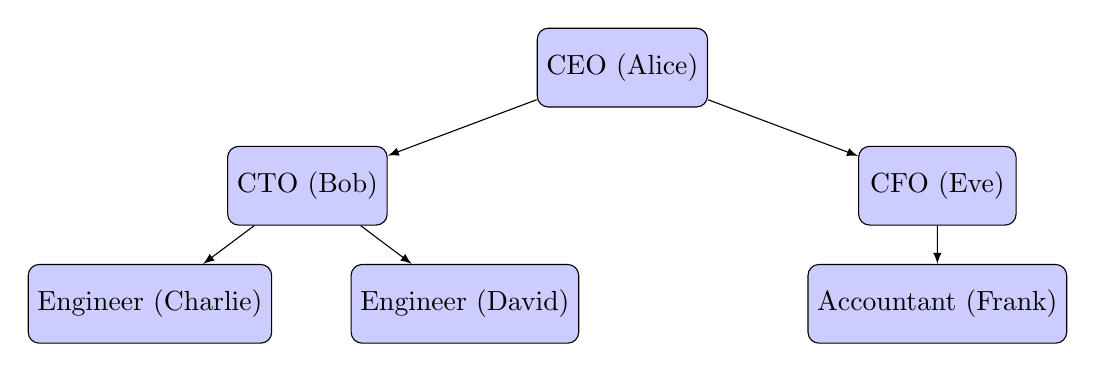
\begin{tikzpicture}[
		level 1/.style={sibling distance=80mm},
		level 2/.style={sibling distance=40mm},
		edge from parent/.style={draw,-latex},
		every node/.style={draw,rounded corners,fill=blue!20,minimum width=2cm,minimum height=1cm,align=center}
		]
		
		\node {CEO (Alice)}
		child {node {CTO (Bob)}
			child {node {Engineer (Charlie)}}
			child {node {Engineer (David)}}
		}
		child {node {CFO (Eve)}
			child {node {Accountant (Frank)}}
		};
		
	\end{tikzpicture}
\end{center}


\subsection{Contoh Input dan Output}

\begin{itemize}
	\item \textbf{Mencari Atasan dari Charlie:} Bob
	\item \textbf{Mencari Atasan Hingga CEO dari David:} [Bob, Alice]
	\item \textbf{Mencari Bawahan Langsung dari Bob:} [Charlie, David]
	\item \textbf{Mencari Semua Bawahan dari Bob:} [Charlie, David]
\end{itemize}

\subsection{Petunjuk:}

\begin{itemize}
	\item Representasikan struktur organisasi menggunakan struktur data tree, di mana setiap node memiliki atribut nama karyawan dan referensi ke bawahan (child nodes).
	\item Gunakan traversal pohon, baik depth-first search (DFS) atau breadth-first search (BFS), untuk menyelesaikan fungsi-fungsi pencarian atasan dan bawahan.
	\item Untuk fungsi yang mencari semua bawahan, Anda bisa menggunakan algoritma rekursif untuk mengunjungi seluruh subtree dari karyawan yang bersangkutan.
	\item Uji setiap fungsi dengan beberapa nama karyawan yang berbeda dalam struktur organisasi untuk memastikan bahwa fungsi-fungsi tersebut bekerja dengan baik.
\end{itemize}

Tugas Anda adalah mengimplementasikan fungsi-fungsi tersebut dalam bahasa pemrograman Java.

\subsection{Kode Awal:}
\begin{lstlisting}[style=JavaStyle]
	import java.util.ArrayList;
	import java.util.List;
	
	// Class representing a node in the tree
	class TreeNode {
		private String position;  // Job position (e.g., CEO, CTO, Engineer)
		private String name;      // Name of the person (e.g., Alice, Bob)
		private List<TreeNode> children;  // List of child nodes (subordinates)
		
		public TreeNode(String position, String name) {
			this.position = position;
			this.name = name;
			this.children = new ArrayList<>();
		}
		
		public void addChild(TreeNode child) {
			children.add(child);
		}
		
		public List<TreeNode> getChildren() {
			return children;
		}
		
		public String getPosition() {
			return position;
		}
		
		public String getName() {
			return name;
		}
		
		@Override
		public String toString() {
			return position + " (" + name + ")";
		}
		
		// Recursive function to print the tree structure
		public void printTree(String prefix) {
			System.out.println(prefix + toString());
			for (TreeNode child : children) {
				child.printTree(prefix + "    ");
			}
		}
	}
	
	// Main class to demonstrate the tree structure
	public class Main {
		public static void main(String[] args) {
			// Create the root node (CEO)
			TreeNode ceo = new TreeNode("CEO", "Alice");
			
			// Create CTO node and its children
			TreeNode cto = new TreeNode("CTO", "Bob");
			TreeNode engineer1 = new TreeNode("Engineer", "Charlie");
			TreeNode engineer2 = new TreeNode("Engineer", "David");
			cto.addChild(engineer1);
			cto.addChild(engineer2);
			
			// Create CFO node and its child
			TreeNode cfo = new TreeNode("CFO", "Eve");
			TreeNode accountant = new TreeNode("Accountant", "Frank");
			cfo.addChild(accountant);
			
			// Add CTO and CFO to CEO
			ceo.addChild(cto);
			ceo.addChild(cfo);
			
			// Print the tree structure
			ceo.printTree("");
		}
	}
\end{lstlisting}


\section{Soal \textit{Graph}}

Diberikan sebuah graph yang merepresentasikan beberapa kota besar di dunia beserta jarak antar kota-kota tersebut. Setiap node merepresentasikan sebuah kota, dan setiap edge (sisi) merepresentasikan jarak antara dua kota.


\begin{enumerate}
	\item \textbf{Cari Jarak dari Kota A ke Kota B} \\
	Buatlah fungsi yang menerima dua parameter, yaitu nama kota A dan kota B, dan mengembalikan jarak antara kedua kota tersebut berdasarkan graph yang sudah diberikan.
	
	\item \textbf{Tampilkan Kota-Kota yang Dilalui dari Kota A ke Kota B} \\
	Buat fungsi yang menampilkan daftar kota-kota yang dilalui dalam perjalanan dari kota A ke kota B berdasarkan rute yang ada di graph.
	
	\item \textbf{Cari Jalur Terpendek dari Kota A ke Kota B} \\
	Buat fungsi untuk mencari dan menampilkan jalur terpendek dari kota A ke kota B, serta menampilkan total jaraknya.
	
	\item \textbf{Cari Jalur Terpanjang dari Kota A ke Kota B} \\
	Buat fungsi untuk mencari dan menampilkan jalur terpanjang dari kota A ke kota B, serta menampilkan total jaraknya.
\end{enumerate}

Berikut adalah contoh graph yang merepresentasikan beberapa kota besar di dunia beserta jarak antar kota:

\begin{center}
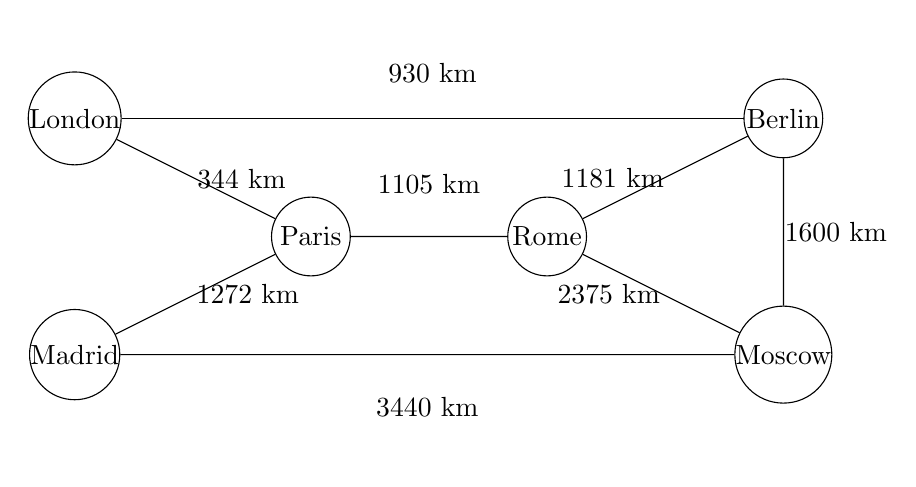
\begin{tikzpicture}[scale=1.5, every node/.style={circle, draw, minimum size=1cm, inner sep=0pt}]
	% Define the nodes (cities)
	\node (London) at (0, 0) {London};
	\node (Paris) at (2, -1) {Paris};
	\node (Berlin) at (6, 0) {Berlin};
	\node (Rome) at (4, -1) {Rome};
	\node (Madrid) at (0, -2) {Madrid};
	\node (Moscow) at (6, -2) {Moscow};
	
	% Draw edges with distances
	\draw (London) -- (Paris) node[midway, right, draw=none] {344 km};
	\draw (London) -- (Berlin) node[midway, above, draw=none] {930 km};
	\draw (Paris) -- (Rome) node[midway, above, draw=none] {1105 km};
	\draw (Berlin) -- (Rome) node[midway, left, draw=none] {1181 km};
	\draw (Paris) -- (Madrid) node[midway, right, draw=none] {1272 km};
	\draw (Berlin) -- (Moscow) node[midway, right, draw=none] {1600 km};
	\draw (Rome) -- (Moscow) node[midway, left, draw=none] {2375 km};
	\draw (Madrid) -- (Moscow) node[midway, below, draw=none] {3440 km};
\end{tikzpicture}
\end{center}
\[
\begin{array}{c|c|c}
	\textbf{Kota A} & \textbf{Kota B} & \textbf{Jarak (km)} \\
	\hline
	London & Paris & 344 \\
	London & Berlin & 930 \\
	Paris  & Rome  & 1105 \\
	Berlin & Rome  & 1181 \\
	Paris  & Madrid & 1272 \\
	Berlin & Moscow & 1600 \\
	Rome   & Moscow & 2375 \\
	Madrid & Moscow & 3440 \\
\end{array}
\]

\subsection{Petunjuk:}

\begin{itemize}
	\item Gunakan struktur data \textit{graph} untuk menyimpan kota-kota beserta jarak antar kota.
	\item Implementasikan tiga kelas berikut:
	\begin{itemize}
		\item \textbf{Graph}: Kelas ini merepresentasikan keseluruhan graph dan menyimpan node dan edge.
		\item \textbf{Node}: Kelas ini merepresentasikan kota, yang memiliki atribut seperti nama kota.
		\item \textbf{Edge}: Kelas ini menghubungkan dua kota (node) dan memiliki atribut untuk menyimpan jarak antara kedua kota tersebut.
	\end{itemize}
	\item Buat fungsi untuk mencari jalur terpendek dari 2 kota.
	\item Lakukan hal yang sama untuk mencari jalur terpanjang antara 2 kota.
	\item Tampilkan juga kota apa saja yang dilewati.
\end{itemize}

Tugas Anda adalah mengimplementasikan fungsi-fungsi tersebut dalam bahasa pemrograman Java.

\subsection{Kode Awal:}
\begin{lstlisting}[style=JavaStyle]
	class Node {
		private String cityName;
		
		public Node(String cityName) {
			this.cityName = cityName;
		}
		
		public String getCityName() {
			return cityName;
		}
		
		@Override
		public String toString() {
			return cityName;
		}
	}
	
	class Edge {
		private Node node1;
		private Node node2;
		private int distance; // Distance between the two nodes
		
		public Edge(Node node1, Node node2, int distance) {
			this.node1 = node1;
			this.node2 = node2;
			this.distance = distance;
		}
		
		public Node getNode1() {
			return node1;
		}
		
		public Node getNode2() {
			return node2;
		}
		
		public int getDistance() {
			return distance;
		}
		
		@Override
		public String toString() {
			return node1 + " <--> " + node2 + ": " + distance + " km";
		}
	}
	
	import java.util.ArrayList;
	import java.util.List;
	
	class Graph {
		private List<Node> nodes;
		private List<Edge> edges;
		
		public Graph() {
			nodes = new ArrayList<>();
			edges = new ArrayList<>();
		}
		
		public void addNode(Node node) {
			nodes.add(node);
		}
		
		public void addEdge(Node node1, Node node2, int distance) {
			Edge edge = new Edge(node1, node2, distance);
			edges.add(edge);
		}
		
		public void displayGraph() {
			for (Edge edge : edges) {
				System.out.println(edge);
			}
		}
	}
	
	public class Main {
		public static void main(String[] args) {
			// Create a new graph
			Graph graph = new Graph();
			
			// Create nodes (cities)
			Node london = new Node("London");
			Node paris = new Node("Paris");
			Node berlin = new Node("Berlin");
			Node rome = new Node("Rome");
			Node madrid = new Node("Madrid");
			Node moscow = new Node("Moscow");
			
			// Add nodes to the graph
			graph.addNode(london);
			graph.addNode(paris);
			graph.addNode(berlin);
			graph.addNode(rome);
			graph.addNode(madrid);
			graph.addNode(moscow);
			
			// Add edges with distances
			graph.addEdge(london, paris, 344);
			graph.addEdge(london, berlin, 930);
			graph.addEdge(paris, rome, 1105);
			graph.addEdge(berlin, rome, 1181);
			graph.addEdge(paris, madrid, 1272);
			graph.addEdge(berlin, moscow, 1600);
			graph.addEdge(rome, moscow, 2375);
			graph.addEdge(madrid, moscow, 3440);
			
			// Display the graph
			graph.displayGraph();
		}
	}
\end{lstlisting}



